% !TEX encoding = UTF-8 Unicode

\documentclass[a4paper]{article}

\usepackage[utf8]{inputenc}
\usepackage[T1]{fontenc}

\usepackage{graphicx}
\usepackage{amsmath}
\usepackage{xcolor}
\usepackage{pgffor} %provides the command \foreach
\usepackage{mathtools} %provides \clap and mathmode versions of \mathrlap, \mathllap, and \mathclap

\newcommand{\bs}[1]{{\rmfamily\color{blue}\textbackslash{}#1}}

\newenvironment{example}[1]{%
\vspace{10pt}
\noindent\textbf{#1}\sffamily\par\vspace{10pt}%
}
{%
\par\vspace{10pt}
}


\newlength{\glyphwd}
\newcommand{\bx}[1]{%
  \bgroup
  \settowidth\glyphwd{#1}%
  \setlength{\fboxrule}{0.1pt}% hairline
  \setlength{\fboxsep}{-0.05pt}%
  \makebox[0pt][l]{\vrule height 0.05pt depth 0.05pt width \glyphwd}%
  \fbox{#1}%
  \egroup
}


\title{A Glimpse on Advanced \LaTeX{}}
\author{J.M. Pérez Pardo}
\date{}


\begin{document}

\maketitle

\tableofcontents

\section{How \LaTeX\ prints glyphs on a page}

Before we answer this question we are going to look at how did a printing press (J. Gutenberg ~1400a.d.) work. The glyphs were molded in small metals blocks like those appearing in Figure~\ref{fig:metalblockschase}. These blocks were used to compose a page by inserting them in a wooden chase, see Figure \ref{fig:metalblockschase}. First building words and then lines. The full chase was then covered with ink and introduced in the \emph{press} to print a page.
%
\begin{figure}[h]
  \hfil\vbox{ \hbox{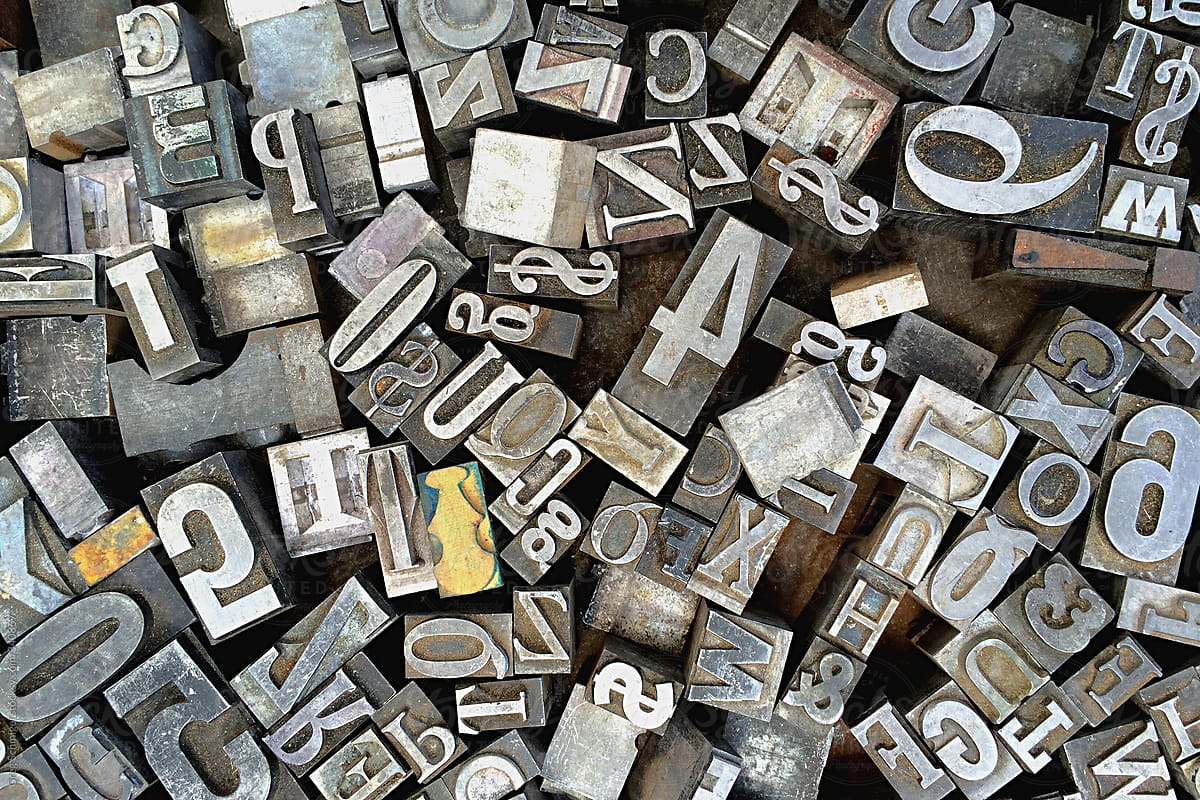
\includegraphics[width=.5\textwidth]{glympse_figures/metal_blocks.jpg}} \vspace{1cm}}\hskip 0pt plus 0.5fil 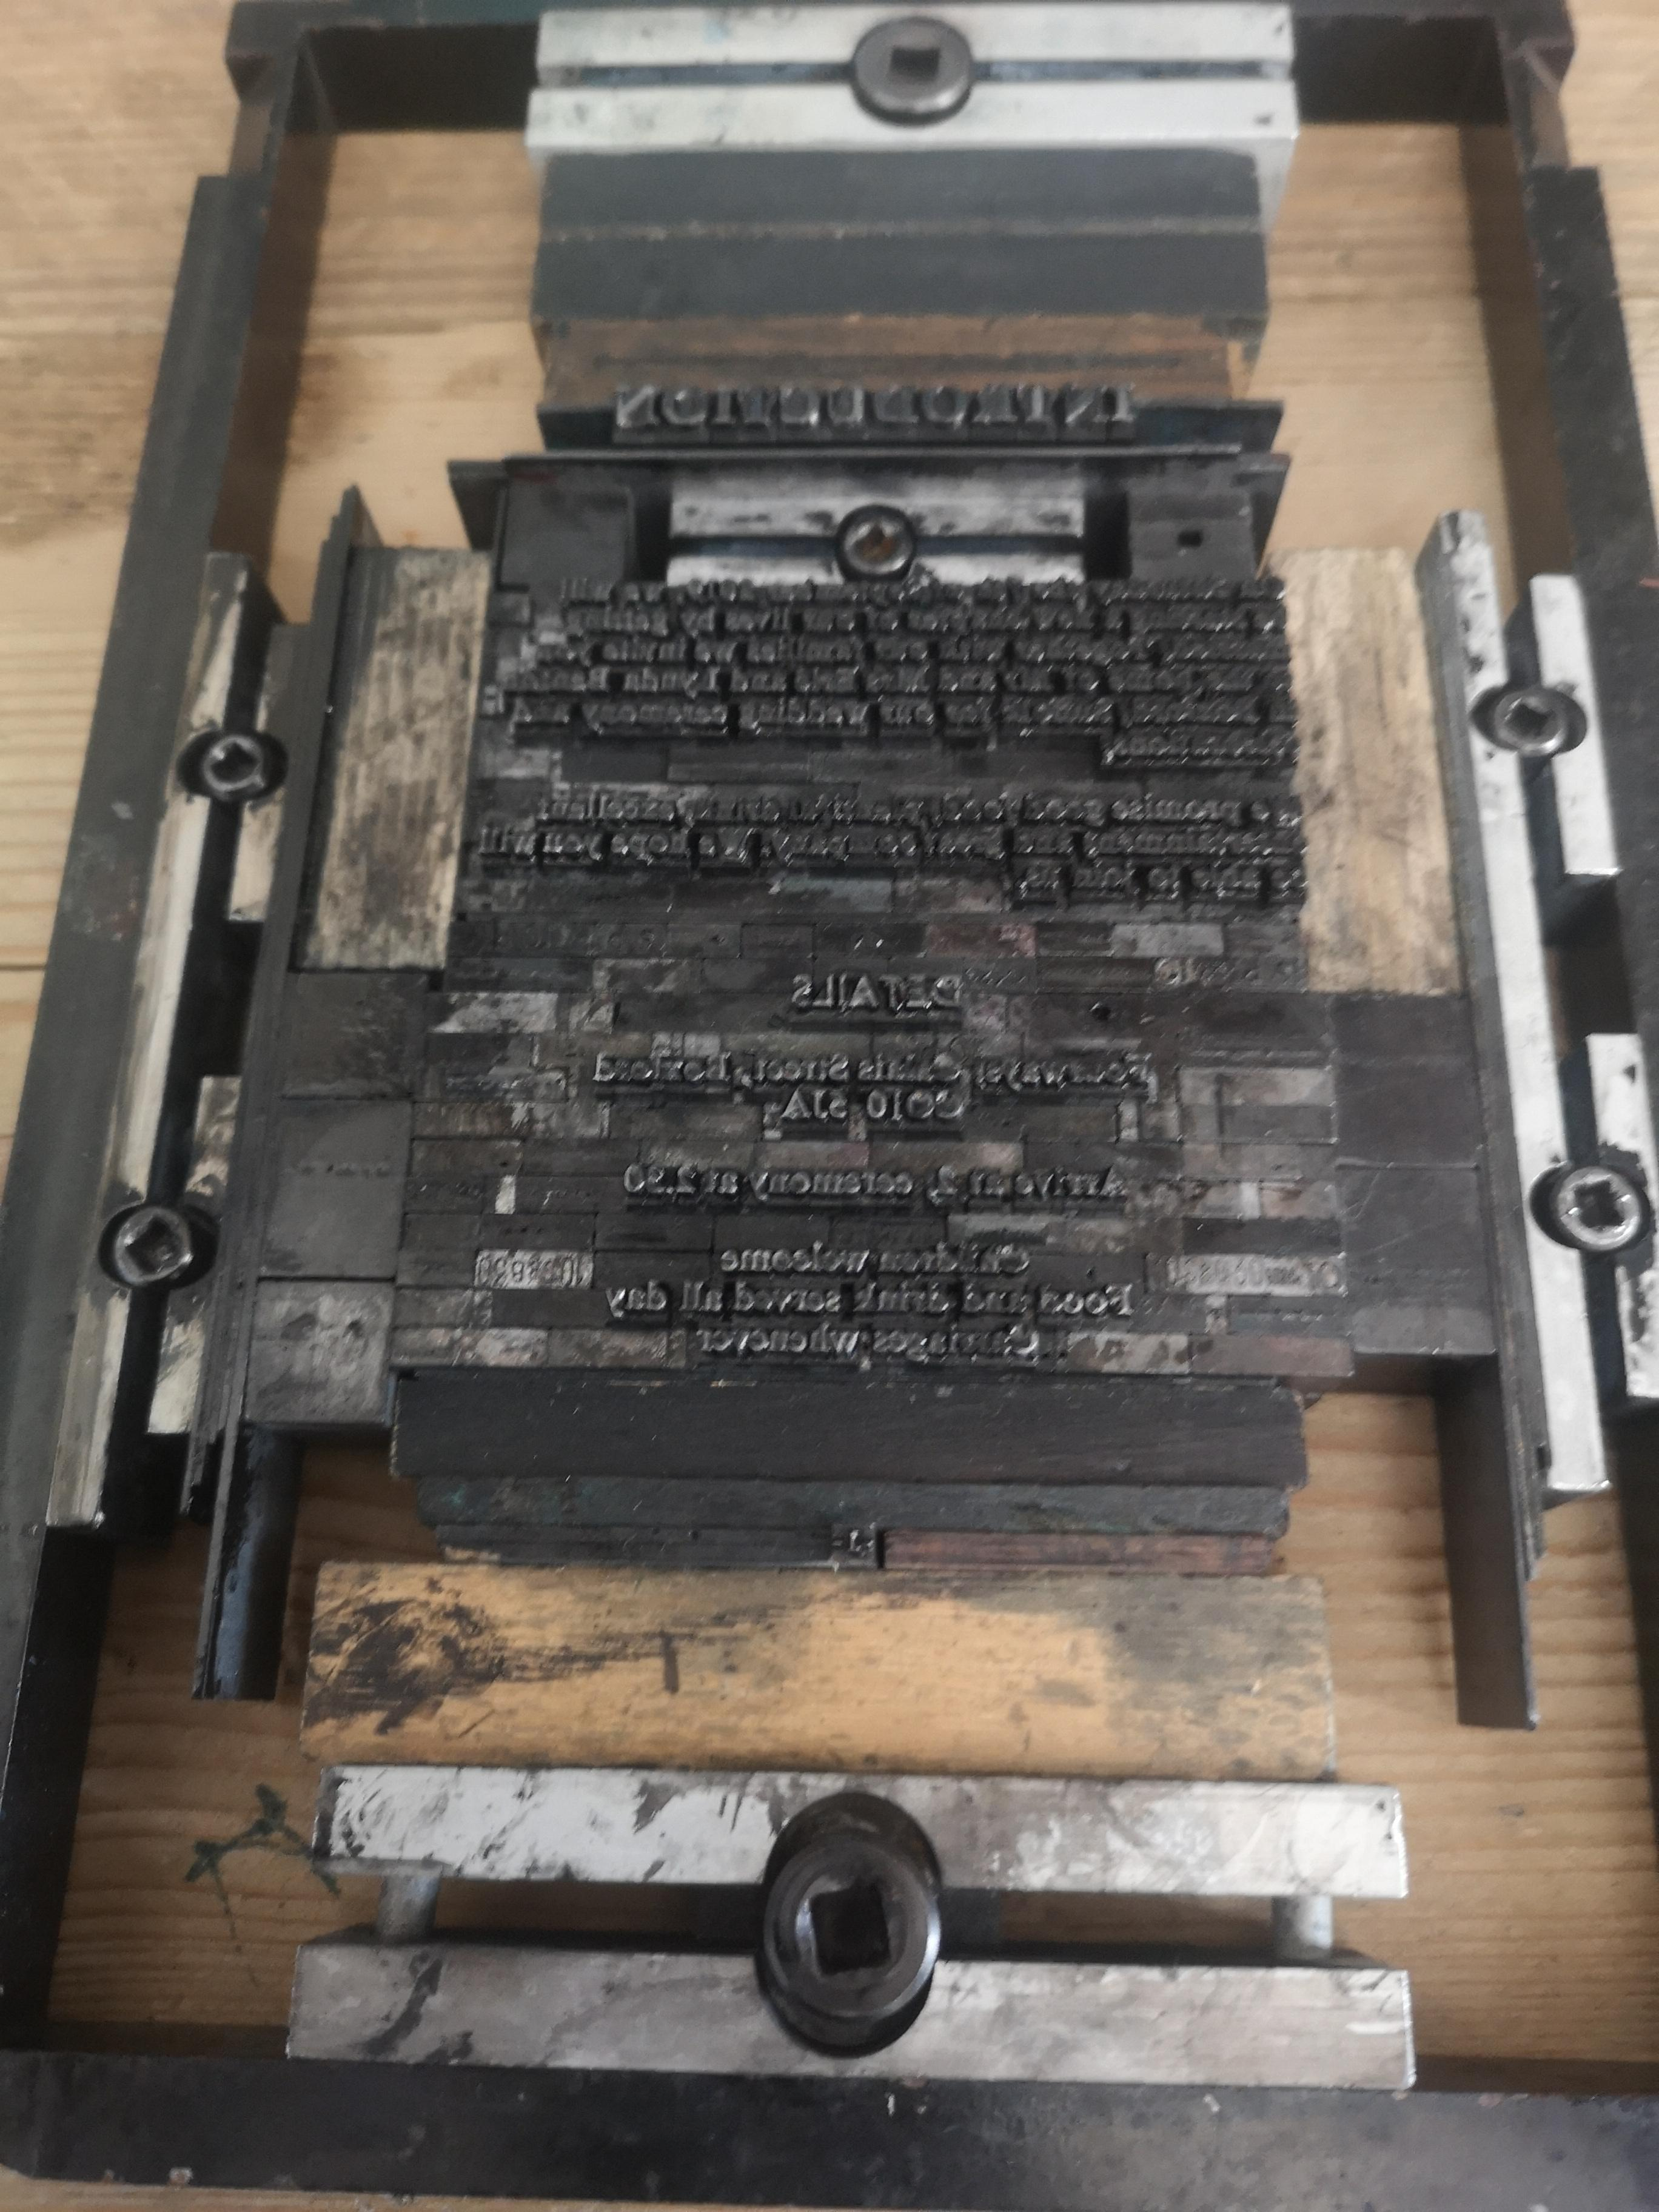
\includegraphics[width=.4\textwidth]{glympse_figures/chase.jpg}\hfil
  \caption{\emph{Left}: Metal blocks and chase used in a printer press. \emph{Right}: Chase where the metal blocks are inserted}\label{fig:metalblockschase}
\end{figure}
%

\TeX\ (and \LaTeX{}.) does actually a very similar thing to compose a document. Each glyph is contained in an invisible container called \emph{box} that has a rectangular shape. This box has given dimensions, \emph{width}, \emph{height} and \emph{depth} and determines how much space does it take. The \emph{ink} of the glyph is adjusted with respect to the box. The ink might even lie outside of the box. Actually \TeX\ does not care about the ink. All that matters to it are the boxes and their alignment. How the ink is placed with respect to the box is decided by the persons how designed the different fonts. When parsing the document, \TeX\ construct words putting all these boxes together and building bigger boxes. 

\section{Boxes}

A box is a rectangular shaped object that has three numbers (also called dimensions) associated to it, \emph{width}, \emph{height} and \emph{depth}. These dimensions determine how big a box is and what its relative position to neighboring boxes will be.  The structure of a box can be seen in Figure~\ref{fig:box}. The baseline determines the imaginary line where characters lie. The height determines how high a character lies above the baseline and the depth determines how much it \emph{hangs} from the baseline. For instance, the box of the glyph ``h'' has a bigger height than the box of the glyph ``a'' and both of them have 0 depth. The box of the glyph ``g'' has the same height than the box of the glyph ``a'' but non-zero depth.
%
\begin{figure}[h]
  \hfil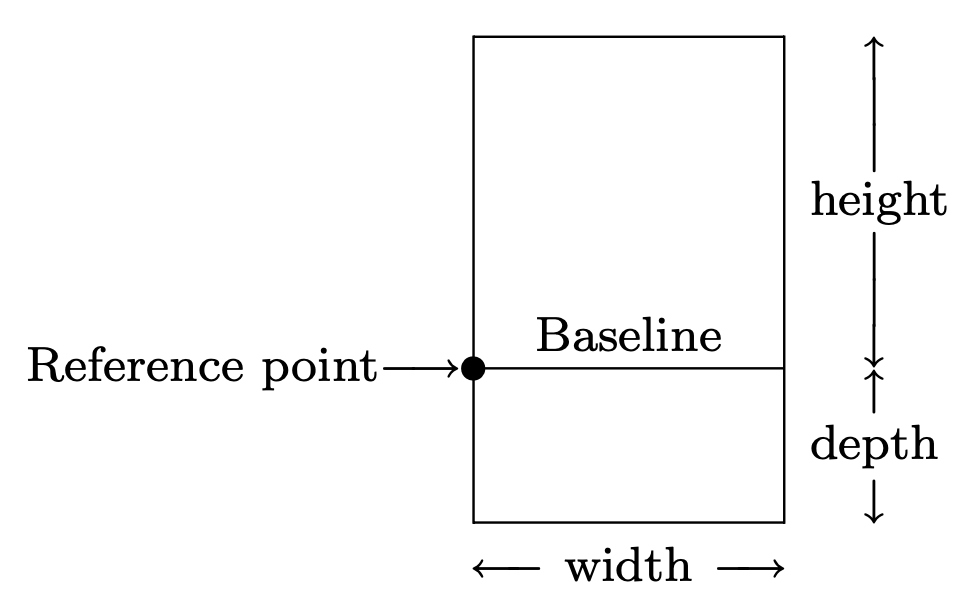
\includegraphics[width=.7\textwidth]{glympse_figures/box.png}\hfil
  \caption{A box and its dimensions. \emph{Source}: The \TeX{}book \cite{Knuth1990}\label{fig:box}}
\end{figure}

The macro \bs{bx} defined in the preamble displays the margins of the boxes so that we can have a look at the dimensions directly:\\

\hfil\foreach \i in {x, M, f, g, ), p, {\itshape f}}{\bx{\i}\hfil}\\

\noindent Actually these are too small to be appreciated in depth so I will use a larger font. This is done with the \bs{Huge} command.\\

\hfil\foreach \i in {x, M, f, g, ), p, {\itshape f}}{\bx{\Huge \i}\hfil}\\

\noindent Notice that ``x'', ``M'', ``f'' have no depth while ``g'', ``)'', ``p'', ``\textit{f}'' have. In addition, notice that the ink of the italic shape of the letter ``f'' lies outside the box. This is something usual in italic fonts. Otherwise the characters in a word would be too separated from each other. Notice also how each character has a different width.


\section{Horizontal and vertical modes. How \LaTeX{} puts boxes together and prints pages.}

Now that we know how \LaTeX{} understands each character we are going to get an idea of how it does to build the page. When producing the document the source file is split into text units which are paragraphs. Each paragraph will end up being a paragraph in the final document. When the parser begins reading a paragraph it knows that the paragraph ends when a \bs{par} command is found. This might be the first time that we see this command because it is rarely typed in the source code. The reason is that a blank line in the source code, two end of line characters with possibly white spaces between them, is interpreted automatically like the \bs{par} command. The next two paragraphs are an example of this. Check the source code. There is no blank line in between the next two paragraphs but a \bs{par} command.

\begin{example}{Two paragraphs separated by a \bs{par}}
No one expects the Spanish Inquisition! Our chief weapon is surprise, fear and surprise; two chief weapons, fear, surprise, and ruthless efficiency! [a \bs{par} command is here and no blank line]\par Er, among our chief weapons are: fear, surprise, ruthless efficiency, and near fanatical devotion to the Pope! Um, I'll come in again
\end{example}

Whenever a paragraph starts or ends several things happen. There are some obvious formatting operations that occur, like adding the indentation on the first line of including extra space between the first line of a paragraph and the last line of the previous one. But there are many other things that occur internally and we will give a brief description of what happens with them. Before a paragraph starts the parser is in the so called \emph{vertical mode}. When the parser meets the first character of a paragraph it switches to horizontal mode and starts putting boxes together. First it collects all the non-white space characters that he finds up to the next white space character. The boxes are aligned at their reference points, so that they share the baseline. Once the word is complete a new box is defined that has height and depth the biggest height and depth of the boxes that compose it, and width the total sum of the widths of all the boxes. This is illustrated next with the word ``Perspective''.\\

\noindent\hfil
\includegraphics{glympse_figures/word.pdf}\hfil
\includegraphics{glympse_figures/word_boxed.pdf}\hfil\\

\noindent The different boxes of the words are then put together. Between the words, white space is added. As you can see in the example below white space is not a box of a given width without ink. This white space is called \emph{glue} and is what allows \TeX{} to print the justified blocks of text. We will speak about \emph{glue} later.\\

\noindent\hfil
\includegraphics{glympse_figures/sentence.pdf}\hfil\\

\noindent \TeX{} will continue to do so until it has finished parsing the full paragraph. At this time what \TeX{} has is a very long line representing the paragraph. It is now time to break the paragraph into lines. The \emph{glue}, i.e., the white space between words, has not a fixed length but instead can stretch or shrink to make the lines exactly as long as needed. \TeX{} has a complicated algorithm, cf. \cite[Chapter~14]{Knuth1990}, to decide where are the optimal points to break the paragraph into lines such that the outcome is as visually pleasant as possible. We are not going to enter in the details of this algorithm but at the end of this section we will discuss some basic things that will allow us to tune how it works.
After the paragraph is broken into lines the parser goes into \emph{vertical mode}. This time, the boxes that make the lines are put vertically one after the other and there is also some \emph{glue} inserted between these boxes. You can get an idea with the following picture.\\ 

\noindent\hfil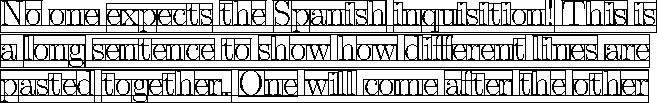
\includegraphics{glympse_figures/paragraph_boxed.pdf}\hfil\\

\noindent All that is missing is to stretch the glue to make all line boxes have the same length. The parser continues then in \emph{vertical mode} until the next paragraph starts. When there are enough lines to fit a page it is \emph{shipped} for printing. In principle \TeX{} could  use a similar algorithm than it uses for breaking a paragraph into lines to split the document into pages but it doesn't. When the lines have enough length to fit the page they are stretched or shrunk for the best output and the page is closed for shipping. This was done so because of memory considerations. Notice that the full document should be in memory to accomplish this and for a very large document this could be a problem.

We are going to give now some hints in how the paragraph breaking algorithm works. The fundamental idea is that breaking the paragraph at a point has a cost. This was called by D.E.~Knuth the \emph{badness}. The algorithm considers many possibilities of breaking the paragraph into lines and chooses the one with the minimum \emph{badness}. This works roughly as follows. If a line has to be stretched or shrunk to fit the page it gets a \emph{penalty} depending on how much it had to be stretched or shrunk. Other operations like hyphenating a word also have a \emph{penalty} and so on. The interesting thing about this is that penalties can be set by hand to force or prevent \TeX{} to take a line break. This is done with the \bs{penalty} command. Normally you do not need to take care about this but on occasions you might feel that a certain break is not appropriate and we will see what can be done in those cases. Typical penalties handled by \TeX{} are in a range between 10 and 10. A penalty of 10000  (\bs{penalty 10000}) or more is considered to be so large that \TeX{} will never break there. Penalties can be negative too. This makes certain breakpoints to be more desirable than others as the total badness will be diminished if the break point happens there. A penalty of -10000 (\bs{penalty -10000}) is considered to be so low that \TeX{} will always break there.\\

\begin{example}{A paragraph to be used as reference to see the effect of adding penalties.}
No one expects the Spanish Inquisition! Our chief weapon is surprise, fear and surprise; two chief weapons, fear, surprise, and ruthless efficiency! Er, among our chief weapons are: fear, surprise, ruthless efficiency, and near fanatical devotion to the Pope! Um, I'll come in again\dots
\end{example}

\noindent As you can see the points that have been chosen by \TeX{} to break the lines are after the words ``and'', ``our'', and ``to''. The next paragraph has a penalty of 10000 after the word ``our''.

\begin{example}{The paragraph above with a penalty of 10000 after the word ``our''}
No one expects the Spanish Inquisition! Our chief weapon is surprise, fear and surprise; two chief weapons, fear, surprise, and ruthless efficiency! Er, among our{\penalty10000} chief weapons are: fear, surprise, ruthless efficiency, and near fanatical devotion to the Pope! Um, I'll come in again\dots
\end{example}

\noindent You can see that the break didn't occur after the word ``our'' but there were more changes in the paragraph. To avoid stretching that line too much \TeX{} changed the breaks of the other lines too. We want to keep the ``and'' as the breaking point of the first paragraph so let us add a penalty of -10000 after the ``and'' and see what happens.

\begin{example}{The paragraph above with a penalty of 10000 after the word ``our'' and a penalty of -10000 after the word ``and''}
No one expects the Spanish Inquisition! Our chief weapon is surprise, fear and{\penalty-10000} surprise; two chief weapons, fear, surprise, and ruthless efficiency! Er, among our{\penalty10000} chief weapons are: fear, surprise, ruthless efficiency, and near fanatical devotion to the Pope! Um, I'll come in again\dots
\end{example}

\noindent This time the white space of the second line was stretched a lot to fit the line width. Notice that not all white spaces were stretched by the same amount\dots We will understand why this is so when we learn about glue in the next section. Let us consider a final example with a penalty -10000 after the word ``fear,'', that is, about at the middle of one optimal line.

\begin{example}{The paragraph above with a penalty of -10000 after the word ``fear,''.}
No one expects the Spanish Inquisition! Our chief weapon is surprise, fear and surprise; two chief weapons, fear,{\penalty-10000} surprise, and ruthless efficiency! Er, among our chief weapons are: fear, surprise, ruthless efficiency, and near fanatical devotion to the Pope! Um, I'll come in again\dots
\end{example}

\noindent As expected we are forcing a line break there, but the line is stretched by a fairly large amount. Actually, this is almost what \TeX{} to force a line break when one types \bs{\bs{ }}, but the stretching needs to be corrected.

\section{The \emph{glue} and spacing in \LaTeX}

All the spacing commands in \LaTeX{} are related with \emph{glue}. When parsing the document any amount of spaces between characters is substituted by \emph{glue} and a single end of line character is transformed by the parser into a white space and therefore also \emph{glue}. Actually the name \emph{glue} is not very descriptive of what it does and the name \emph{spring} would be more appropriate. This is how D.E.~Knuth puts it: ``\emph{Once you understand \TeX{}’s concept of glue, you may well decide that it was misnamed; real glue doesn’t stretch or shrink in such ways, nor does it contribute much space between boxes that it welds together. Another word like ``spring'' would be much closer to the essential idea, since springs have a natural width, and since different springs compress and expand at different rates under tension. But whenever the author has suggested changing \TeX{}’s terminology, numerous people have said that they like the word “glue” in spite of its inappropriateness; so the original name has stuck.}'' 

There are two types of \emph{glue}. One for the horizontal mode and one for the vertical mode. The primitive \TeX{} commands for including them are \bs{hskip} and \bs{vskip}. They add glue respectively in the horizontal and the vertical mode. Glue accepts three parameters, which must be \emph{dimensions}. That is a number following a unit of measure like \texttt{pt} (points), \texttt{cm} (centimeters), \texttt{ex} (the width of a small x in the current font), \texttt{em} (the width of a capital M in the current font) and others.\\

\bs{hskip}{\ttfamily~<\textsf{\itshape dimen}> plus <\textsf{\itshape dimen}> minus <\textsf{\itshape dimen}>}

\bs{vskip}{\ttfamily~<\textsf{\itshape dimen}> plus <\textsf{\itshape dimen}> minus <\textsf{\itshape dimen}>}\\

\noindent The first dimension gives the fix space that the glue will take. The second dimension, after the ``plus'', determines how much it can stretch and the third one, after the ``minus'', how much it can shrink. For example, in the source code you could write\\

{\ttfamily WORD \bs{hskip} 2em plus 1ex minus 2pt WORD}\\

Which results in\\

WORD \hskip 2em plus 1ex minus 2pt WORD \\

This means that each \emph{glue} between words has a determined amount of stretchability or shrinkability. When a box has to be stretched (or shrunk) each glue in it adds (or substracts) to each fixed length a quantity proportional to its glue plus (minus) dimension to get the desired length. For instance, after punctuation marks the \emph{glue} is more stretchable than between words and so is \emph{glue} after a dot than after a comma. This explains the behaviour of the stretching in the examples of the previous section.

In addition to the dimensions mentioned above, \TeX{} has defined \textbf{three different types of infinity}. Each one of them is infinitely larger than the previous one. These are called \texttt{fil}, \texttt{fill} and \texttt{filll} in increasing order of infinity. These infinities can be used as the dimension of the stretching or shrinking quantity in \emph{glue}. In essence they provide an infinite amount of stretchability that fills the line, justifying their name. Below some examples on how this works.

\begin{example}{Using \emph{glue} with infinite stretchability}
Below we have several examples. There is a line with the source code and directly below it is the output that it produces.\\

\verb!word \hskip 0pt plus 1fil minus 0pt word!:

word \hskip 0pt plus 1fil minus 0pt word\\

\verb!word \hskip 0pt plus 1fill minus 0pt word!:

word \hskip 0pt plus 1fill minus 0pt word\\

\verb!word \hskip 0pt plus 1filll minus 0pt word!:

word \hskip 0pt plus 1filll minus 0pt word\\

\verb!word \hskip 0pt plus 1fill  word  \hskip 0pt plus 1fill word!:

word \hskip 0pt plus 1fill  word  \hskip 0pt plus 1fill word\\

\verb!word \hskip 0pt plus 1fill  word  \hskip 0pt plus 2fill word!:

word \hskip 0pt plus 1fill  word  \hskip 0pt plus 2fill word\\

\verb!word \hskip 0pt plus 1filll  word  \hskip 0pt plus 10fill word!:

word \hskip 0pt plus 1filll  word  \hskip 0pt plus 10fill word\\


\end{example}

We can see that a greater infinity type neglects the presence of lower infinities. Infinities of the same type will be weighted according to the amount of it in the line. There is just one point that should raise our attention tight now. Why doesn't the infinite stretchability of the first example push the right word to the end of the line like in the other cases? The answer has to do with what \TeX{} does at the end of a paragraph to prevent the last line to stretch. At the end of a paragraph automatically an ``\bs{hskip} {\ttfamily 0pt plus~1fil minus~0pt}'' is inserted to keep the line short. The second word is pushed at its two sides by equally weighted infinite \emph{glue}. That is why it remains near the middle of the line.

There are some macros which are shorthand for this infinite stretchable \emph{glue}. For instance \bs{hfil} is defined as \bs{hskip} {\ttfamily 0pt plus~1fil minus~0pt} and equivalently \bs{hfill}, \bs{vfil} and \bs{vfill}. There is no macro for the greatest infinity because it is rarely used. There are also macros to define fixed, i.e., non stretchable/shrinkable \emph{glue}. These are \bs{hspace}\{<\textsf{\itshape dimen}>\} and \bs{vspace}\{<\textsf{\itshape dimen}>\}. The former is defined by \bs{hskip}{\ttfamily~<\textsf{\itshape dimen}> plus~0pt minus~0pt} and the latter is defined equivalently. In this document I have used these macros and also some \emph{glue} to tune the adjustment of the figures. Have a look at them in the source file to see what effect they had in the final layout. 

There is still one important  thing to discuss and is that vertical \emph{glue} takes effect only during the vertical mode. When \TeX{} is in horizontal mode and encounters a \bs{vspace} command it is not inserted immediately but after the line that contains it and will be used in vertical mode to spread the lines. Check the following example where a \bs{vspace} command is used in the middle of the paragraph. Intuitively one would expect that after the command the rest of the text would have been shifted, but this is not what happens.

\newpage\begin{example}{A \bs{vspace}\{1cm\} is inserted after ``Inquisition!''}
No one expects the Spanish Inquisition!\vspace{1cm}Our chief weapon is surprise, fear and surprise; two chief weapons, fear, surprise, and ruthless efficiency! 

Er, among our chief weapons are: fear, surprise, ruthless efficiency, and near fanatical devotion to the Pope! Um, I'll come in again\dots
\end{example}

To prevent this behaviour use vertical \emph{glue} at the beginning or end of a paragraph, or between paragraphs.


\section{Special commands to manipulate boxes}

It is time know to learn some commands that allow to manipulate boxes. Knowing this allows for fine tuning of placement, in particular in formulas. \LaTeX{} does a great job at typesetting but not all the cases are covered by the programers and many cases need to be adjusted by hand. Many of these situations can be addressed easily by knowing the following commands. In addition, they can be used to defined many useful macros that can be adapted to many situations. We will learn this in the examples. Remember that arguments in square brackets represent optional arguments, they might be given or not.  Each command comes with some examples. The boxes are typeset using the \bs{bx} command defined in the preamble. They would not be seen otherwise.

\begin{description}
  \item[\bs{hbox}\{contents\}] This is a \TeX{} primitive. It creates a box with the contents parsed in \emph{horizontal mode}. It should be avoided in favour of \bs{mbox} except in special situations. This box is unbreakable once created.\\ Example: \verb!\hbox{Hello}!
  
  \bx{\hbox{Hello}}
  
  \item[\bs{vbox}\{contents\}] This is a \TeX{} primitive. It creates a box with the contents parsed in \emph{vertical mode}. Should be used in situations when one wants to put one box on top of other box. The minipage environment should be used instead of this one. \\ Example: \verb!\vbox{a\\b\\c} \vbox{\hbox{a}\hbox{b}\hbox{c}}!
  
   \bx{\vbox{a\\b\\c}} \bx{\vbox{\hbox{a}\hbox{b}\hbox{c}}}
  
  \item[\bs{mbox}\{contents\}] Essentially like \bs{hbox} with more predictable behaviour. \\ Example: \verb!\mbox{Hello}!
  
  \bx{\mbox{Hello}}
  
  \item[\bs{makebox}{[}width{]}{[}alignment{]}\{contents\}] Like \bs{mbox} but defines a box with given width. The contents can be aligned l,c or r.\\ Example: \verb!\makebox[1em][r]{Hello} \makebox[5em][r]{Hello}!
  
  \bx{\makebox[1em][r]{Hello}} \bx{\makebox[5em][r]{Hello}}
  
  \verb!\makebox[5em][c]{Hello} \makebox[5em][l]{Hello} \makebox[1em][l]{Hello}!
  
   \bx{\makebox[5em][c]{Hello}} \bx{\makebox[5em][l]{Hello}} \bx{\makebox[1em][l]{Hello}}
  
    \item[\bs{newsavebox}\{\bs{name}\}] Creates a \emph{register}, that is, a bin, where one can save a box.
      
  \item[\bs{sbox}\{\bs{name}\}\{contents\}] Creates a box in horizontal mode and saves it in a register (bin) with name \bs{name} that was previously created with \bs{newsavebox}.\\ Example:
  \begin{verbatim}
    \newsavebox{\mybox} 
    \sbox{\mybox}{Hello} 
    The width of \bs{mybox} is \mbox{\the\wd\mybox}. 
    The height of \bs{mybox} is \mbox{\the\ht\mybox}. 
    The depth of \bs{mybox} is \mbox{\the\dp\mybox}.
  \end{verbatim}
  
  \newsavebox{\mybox} 
  \sbox{\mybox}{Hello} 
  The width of \bs{mybox} is \mbox{\the\wd\mybox}. 
  The height of \bs{mybox} is \mbox{\the\ht\mybox}. 
  The depth of \bs{mybox} is \mbox{\the\dp\mybox}.

  
  
  
  
  \item[\bs{savebox}{[}width{]}{[}alignment{]}\{\bs{name}\}\{contents\}] Like \bs{sbox} but adjust the width an alignment like \bs{makebox}.
  
  
  \item[\bs{usebox}\{\bs{name}\}] Prints the box in the register \bs{name}.\\ Example: \verb!\usebox{\mybox}!
  
  \bx{\usebox{\mybox}}
  
  \item[\bs{raisebox}\{dimension\}{[}height{]}{[}depth{]}\{contents\}] raises the contents by dimension. This is, the baseline of the box is moved downwards (or upwards if dimension is negative). The resulting box can have the given height and depth.\\ Example:
  \begin{verbatim}
    \bx{\raisebox{3pt}{Hello}}Hello
    \bx{\raisebox{-3pt}{Hello}}Hello
    \bx{\raisebox{3pt}[5pt][2pt]{Hello}}Hello
  \end{verbatim}
   
  \bx{\raisebox{3pt}{Hello}}Hello
  \bx{\raisebox{-3pt}{Hello}}Hello
  \bx{\raisebox{3pt}[5pt][2pt]{Hello}}Hello
  
  \item[\bs{rule}{[}raise{]}\{width\}\{thickness\}] Creates a box fully covered with ink. If width or thickness is zero it will not be visible in the document, but the box will occupy some space.\\ Example: \verb!\rule{1em}{1ex} \rule{10em}{0pt} \rule[5pt]{1em}{1ex}!
  
  \bx{\rule{1em}{1ex}} \bx{\rule{10em}{0pt}} \bx{\rule[5pt]{1em}{1ex}}
  
  Notice that the rule in the middle can be seen because of the \bs{bx} command. Otherwise it would be invisible.
  
  
  \item[\bs{llap}\{contents\}] Collapses the box of contents to a vertical line at the right. In math mode use \bs{mathllap} instead, which is provided by the {\ttfamily mathtools} package.
  
  
  \item[\bs{clap}\{contents\}] Collapses the box of contents to a vertical line at the center. In math mode use \bs{mathclap} instead. Both commands are provided by the {\ttfamily mathtools} package.
  
  
  \item[\bs{rlap}\{contents\}] Collapses the box of contents to a vertical line at the left. In math mode use \bs{mathrlap} instead, which is provided by the {\ttfamily mathtools} package.\\ Example:
  \begin{verbatim} 
    \hfil
    \llap{\Huge a}
    \hfil
    \rlap{\Huge a}
    \hfil
    \clap{\Huge a}
    \hfil
  \end{verbatim}
  
    \hfil
    \bx{\llap{\Huge a}}
    \hfil
    \bx{\rlap{\Huge a}}
    \hfil
    \bx{\clap{\Huge a}}
    \hfil

 Notice the differences between these formulas. Can you guess what we did in the second one?
 
 $$ X = \sum_{1\leq i \leq j \leq n} X_{ij} \hspace{3cm} X = \sum_{\mathclap{1\leq i \leq j \leq n}} X_{ij}$$
  
  
  \item[\bs{smash}\{contents\}] Collapses the box of contents to a horizontal line at the bottom. Works in text mode and math mode.\\ Example: \verb!\smash{Hello}!
  
  \bx{\smash{Hello}}
  
  \item[\bs{phantom}\{contents\}] Creates a box with the dimensions of contents but without ink. Works in text mode and math mode.\\ Example: \verb!\phantom{Hello}!
  
  \bx{\phantom{Hello}}
  
\end{description}





\bibliographystyle{siam}
\bibliography{my_bibliography.bib}


\end{document}



